\documentclass[fontsize=11pt, paper=a4]{scrartcl}
\usepackage[pass]{geometry}
\usepackage[utf8]{inputenc}
\usepackage[T1]{fontenc}
\usepackage{amsmath, amssymb}
\usepackage[shortlabels]{enumitem}
\usepackage{indentfirst}
\usepackage{mathtools}
\usepackage{fullpage}
\usepackage{graphicx}
\graphicspath{{img/}}

\DeclarePairedDelimiter\ceil{\lceil}{\rceil}
\DeclarePairedDelimiter\floor{\lfloor}{\rfloor}

\setkomafont{disposition}{\rmfamily}

\newlength{\subsectionparindent}
\newlength{\subsectionafterskip}

\RedeclareSectionCommand[
  style     = section,
  font      = \normalfont\bfseries,
  afterskip = \subsectionafterskip,
  indent    = \subsectionparindent,
]{subsection}

\renewcommand{\thesection}{\arabic{subsection}}

\AtBeginDocument{%
  \setlength{\parindent}{\dimexpr2\baselineskip-1ex\relax}%
  \setlength{\subsectionparindent}{\parindent}%
  \setlength{\subsectionafterskip}{\fontdimen2\font plus \fontdimen3\font minus \fontdimen4\font}%
}

\begin{document}
\newgeometry{left=2cm, right=2cm, top=2cm, bottom=2cm, includeheadfoot}

\title{The Art of Computer Programming}
\subtitle{\LARGE Explicit Solutions}
\author{Keaun Moughari} 
\date{\today} 
\maketitle

\setlength{\linewidth}{0.92\linewidth}

\section*{\S \space 1.2.4}\label{part: 1.2.4}
\subsection*{42. re: Lower-bound of internal path length of extended binary trees (p. 400)}\label{num: 42}
\begin{enumerate}[(a), leftmargin=1.5cm]
    \item Prove that $\sum_{k=1}^n a_{k} = na_{n} - \sum_{k=1}^{n-1} k(a_{k+1}-a_{k}), \quad \text{if\space} n > 0.$
        \enlargethispage{0.5cm}
        \vspace{0.5cm}
        \\\textit{Solution:}
        \begin{align*}
            \sum_{k=1}^{n} a_{k}
            &= na_{n} - \sum_{k=1}^{n-1} k(a_{k+1}-a_{k})\\
            &= na_{n} + \sum_{k=1}^{n-1} ka_{k} - \sum_{k=1}^{n-1}ka_{k+1}\\
            &= na_{n} + (a_{1} + 2a_{2} + \cdots + (n-1)a_{n-1})\\
            &\quad - (a_{2} + 2a_{3} + \cdots + (n-2)a_{n-1} + (n-1)a_{n})\\
            &= na_{n} - (n-1)a_{n} + (a_{1} + 2a_{2} + \cdots + (n-1)a_{n-1})\\
            &\quad - (a_{2} + 2a_{3} + \cdots + (n-2)a_{n-1})\\
            &= a_{n} + \sum_{k=1}^{n-1} ka_{k} - \sum_{k=1}^{n-2}ka_{k+1}\\
            &= a_{n} + \sum_{k=0}^{n-2} (k+1)a_{k+1} - \sum_{k=1}^{n-2}ka_{k+1}\\
            &= a_{n} + a_{1} + \sum_{k=1}^{n-2} (k+1)a_{k+1} - \sum_{k=1}^{n-2}ka_{k+1}\\
            &= a_{n} + a_{1} + \sum_{k=1}^{n-2} (k+1)a_{k+1} - ka_{k+1}\\
            &= a_{n} + a_{1} + \sum_{k=1}^{n-2} a_{k+1}\\
            &= a_{n} + a_{1} + \sum_{k=2}^{n-1} a_{k}\\
            &= \sum_{k=1}^{n} a_{k}\\
        \end{align*}
    \item The preceding formula is useful for evaluating certain sums involving the floor function. Prove that, if $b$ is an integer $\ge 2$,
        \begin{equation*}
            \sum_{k=1}^{n} \floor*{\log_b{k}} = (n+1) \floor*{\log_b{n}} - (b^{\floor*{\log_b{n}} + 1} - b) / (b-1).
        \end{equation*}
        \vspace{0.5em}
        \\\textit{Aside:}
        \begin{align*}
            (1) \quad f  &= \floor*{\log_b{n}}; b \ge 2
            &(2) \quad \sum_{1}^{f-1} &= \sum_{j}^{f-1} + \sum_{1}^{j-1}\\
            S_{n-1} &= \sum_{k=1}^{f-1} b^{k}
            &   \Longrightarrow \sum_{j}^{f-1} &= \sum_{1}^{f-1} - \sum_{1}^{j-1}\\
            &= b - b^{\floor*{\log_b{n}}} + \sum_{k=1}^{f-1} b^{k+1}\\
            &= b - b^{\floor*{\log_b{n}}} + b\sum_{k=1}^{f-1} b^{k}\\
            &= b - b^{\floor*{\log_b{n}}} + bS_{n-1}\\
            (1-b)S_{n-1}
            &= b - b^{\floor*{\log_b{n}}}\\
            \Longrightarrow S_{n-1}
            &= \frac{b^{\floor*{\log_b{n}}} - b} {b-1}
        \end{align*}
        \begin{align*}
            \\(3) \quad f  &= \floor*{\log_b{n}}; b \ge 2\\
            S_{n} &= \sum_{k=1}^{n-1} k \text{\space} [k+1 \text{\space is a power of\space} b]\\
            &= \sum_{k=1}^{f} (b^{k} - 1)\\
            &= \sum_{k=1}^{f} b^{k} - \sum_{k=1}^{f} 1\\
            &= \sum_{k=1}^{f} b^{k} - f\\
            &= \left[fb^{f} - \sum_{k=1}^{f-1} k(b^{k+1} - b^{k})\right] - f \quad&\textit{(a)}\\
            &= f(b^{f} - 1) - \sum_{k=1}^{f-1} k(b^{k+1} - b^{k})\\
            &= f(b^{f} - 1) - (b-1)\sum_{k=1}^{f-1} kb^{k}\\
            &= f(b^{f} - 1) - (b-1)\sum_{j=1}^{f-1} \sum_{k=j}^{f-1} b^{k}\displaybreak\\
            &= f(b^{f} - 1) - (b-1)\sum_{j=1}^{f-1} \left(\sum_{k=1}^{f-1} b^{k} - \sum_{k=1}^{j-1} b^{k}\right) \quad&\textit{(2)}\\
            &=  f(b^{f} - 1) - (b-1)\sum_{j=1}^{f-1} \left(\frac {b^{f}-b}{b-1} - \frac{b^{j}-b}{b-1}\right)\\
            &=  f(b^{f} - 1) - (b-1)\sum_{j=1}^{f-1} \left(\frac {b^{f}}{b-1} - \frac{b^{j}}{b-1}\right)\\
            &=  f(b^{f} - 1) - (b-1)\left[\frac{1}{b-1} \left(\sum_{j=1}^{f-1} {b^{f}} - \sum_{j=1}^{f-1} b^{j}\right)\right]\\
            &=  f(b^{f} - 1) - \left(\sum_{j=1}^{f-1} {b^{f}} - \sum_{j=1}^{f-1} b^{j}\right)\\
            &=  f(b^{f} - 1) - \left(b^{f}(f-1) - \sum_{j=1}^{f-1} b^{j}\right)\\
            &=  f(b^{f} - 1) - \left(b^{f}(f-1) - \left(\frac {b^{f}-b}{b-1}\right)\right)\\
            &=  f(b^{f} - 1) - b^{f}(f-1) + \left(\frac {b^{f}-b}{b-1}\right)\\
            &=  fb^{f} - f - fb^{f} + b^{f} + \left(\frac {b^{f}-b}{b-1}\right)\\
            &=  b^{f} - f + \left(\frac {b^{f}-b}{b-1}\right)\\
            (b-1)S_{n}
            &=  (b-1)\left(b^{f} - f\right) + \left(b^{f}-b\right)\\
            &=  b^{f+1} - fb + f - b^{f} + b^{f} - b\\
            &=  b^{f+1} - b - fb + f\\
            &=  b^{f+1} - b - f(b-1)\\
            S_{n}
            &= \left(\frac{b^{f+1} - b}{b-1}\right) - f\\
            \Longrightarrow S_{n}
            &= \frac{b^{\floor*{\log_b{n}}+1} - b}{b-1} - \floor*{\log_b{n}}
        \end{align*}
        \textit{e.o.a.}
        \vspace{0.5cm}
        \\\textit{Solution:}
        \begin{align*}
            \sum_{k=1}^{n} \floor*{\log_b{k}} 
            &= n \floor*{\log_b{n}} - S_{n}\\
            &= n \floor*{\log_b{n}} - \left[\frac{b^{\floor*{\log_b{n}} + 1} - b} {b-1} - \floor*{\log_b{n}}\right]&(3)\\
            &= n \floor*{\log_b{n}} - \frac{b^{\floor*{\log_b{n}} + 1} + b} {b-1} + \floor*{\log_b{n}}\displaybreak\\
            &= (n+1) \floor*{\log_b{n}} - \frac{b^{\floor*{\log_b{n}} + 1} + b} {b-1}\\
        \end{align*}
\end{enumerate}


\section*{\S \space 2.3.4.5}\label{part: 2.3.4.5}
\subsection*{5. re: Generating function of BT with $n$ nodes and internal path length $p$ (p. 404)}\label{num: 5}

\parbox{\linewidth}{
    \qquad Let
    \begin{align*}
        B(w,z) = \sum_{n,p\ge0} b_{np}w^{p}z^{n},
    \end{align*}
    where $b_{np}$ is the number of binary trees with $n$ nodes and internal path length\ 
    $p$.}
\begin{enumerate}[(a), leftmargin=1.5cm]
    \item Find a functional relation that characterizes $B(w,z)$, generalizing $zB(z)^{2} = B(z) - 1$.
    \item Use the result of (a) to determine the average internal path length of a binary tree with $n$\ 
            nodes, assuming that each of the $\frac{1}{n+1} \binom{2n}{n}$ trees is equally probable.
    \item Find the asymptotic value of this quantity.
\end{enumerate}


\section*{\S \space 6.2.1}\label{part: 6.2.1}
\subsection*{25. re: Relation between internal and external nodes in extended BT (p. 425)}\label{num: 25}
\parbox{\linewidth}{
    \qquad Suppose that a binary tree has $a_{k}$ internal nodes and $b_{k}$ external nodes on level $k$,\ 
    for $k=0,1,\dotsc$ (The root is at level zero.) Thus in $\text{Fig.\space} 8$ we have $(a_{0},a_{1},\dotsc,a_{5}) =\
    (1,2,4,4,1,0) \text{\space and\space} (b_{0}, b_{1}, \dotsc, b_{5}) = (0,0,0,4,7,2).$}
\begin{center}
 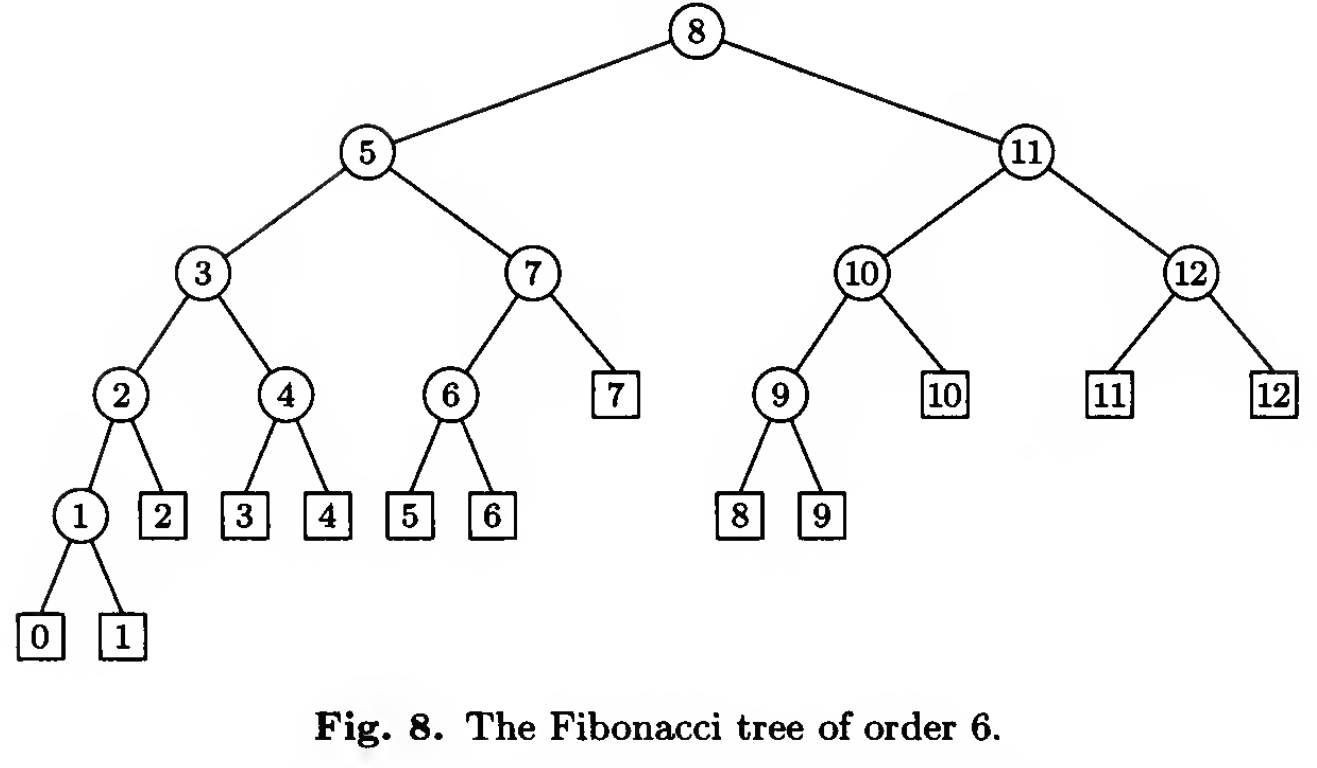
\includegraphics[height=7cm,width=11cm]{figure8.png}
\end{center}
\begin{enumerate}[(a), leftmargin=1.5cm]
    \item Show that a simple algebraic relationship holds between the generating functions $A(z)=\sum_k a_{k}z^{k}$ and $B(z)=\sum_k b_{k}z^{k}$.
    \item The probability distribution for a successful search in a binary tree has the generating function $g(z) = zA(z)/N$,\
            and for an unsuccessful search the generating function is $h(z) = B(z)/(N + 1)$. (Thus in the text’s notation we have \ 
            $C_{N} = \text{mean}(g), C^{'}_{N} = \text{mean}(h)$, and Eq. 2 ($C_{N}=(1+\frac{1}{N})C^{'}_{N}-1$) gives a relation \ 
            between these quantities.) Find a relation between var$(g)$ and var$(h)$.
\end{enumerate}


\end{document}